\section{Analisi}
\subsection{Requisiti}

Il gruppo si pone come obiettivo quello di realizzare la trasposizione videoludica del gioco da tavolo Carcassonne \cite{Carcassonne}. Si tratta di un gioco da 2 a 6 giocatori dove ognuno deve posizionare delle tessere che formano strutture; ovvero strade, praterie, città e monasteri. Su queste strutture possono essere posti dei seguaci, o pedine, con lo scopo di realizzare punti. Chi alla fine della partita avrà totalizzato più punti verrà proclamato vincitore. 

\subsection*{Requisiti funzionali}
Il gioco dovrà permettere ai giocatori che ne partecipano, ognuno identificato univocamente da nome e colore, di piazzare e ruotare tessere ed eventualmente posizionare un seguace. E' necessario:

\begin{itemize}
\item Permettere il posizionamento delle tessere solo in posizioni adiacenti a tessere già piazzate con la quale combaciano i lati
\item Permettere il posizionamento di seguaci su strutture appartenenti alla tessera appena piazzata e senza altri seguaci
\item Calcolare il punteggio dei giocatori, sia nel momento in cui viene chiusa una struttura, che alla fine della partita
\item Permettere la navigazione del campo di gioco
\item Permettere di scartare una tessera che non possa essere piazzata in nessuna delle posizioni libere
\item Permettere di ruotare la tessera prima di piazzarla sul campo di gioco
\item Permettere la selezione del numero dei giocatori e assegnare un nome ed un colore ad ognuno
\item Gestire l'ampliamento e l'unione di praterie, città e strade
\end{itemize}

\subsection*{Requisiti non funzionali}
\begin{itemize}
\item Menù di pausa
\item Visualizzazione grafica e dinamica dei seguaci rimanenti 
\item Pannello per la scelta del colore del giocatore
\item Decorazioni, sfondi e distanziamento fra i vari componenti grafici
\item Supporto di espandibilità futura per l'implementazione di immagini di profilo dei giocatori
\item Supporto alla lingua italiana e inglese
\item Supporto per partecipare alla stessa partita da più interfacce
\item Supporto per future espansioni con l'aggiunta di nuove tessere e seguaci
\end{itemize}

\subsection{Analisi e modello del dominio}

L'analisi e il modello del dominio di Caesena possono essere suddivisi in diversi componenti chiave: i giocatori, le tessere, i seguaci e le strutture. Posizionando un seguace su una struttura, il giocatore ne prende la proprietà, guadagnandone poi i punti alla sua chiusura. A fine partita ogni proprietario di una struttura ne guadagna i punti anche se non chiusa, con il caso speciale delle città nel quale ne guadagna la metà. Una struttura è chiusa quando: 
\begin{itemize}
    \item nel caso delle città, questa non abbia parti non murate. Fa guadagnare al proprietario 2 punti per ogni tessera all'interno della città. Nel caso una tessera contenga uno stemma, allora varrà il doppio
    \item nel caso del monastero, questo sia circondato da 8 tessere. Fa guadagnare al proprietario 1 punto per ogni tessera dalla quale è circondato, più 1 punto per se stesso
    \item nel caso della strada, sia presente un incrocio o un'entrata ad un monastero/città da ambo i lati. Fa guadagnare al proprietario 1 punto per ogni tessera, considerando anche gli estremi
\end{itemize}
Nel caso della prateria, questa non può essere chiusa e fa guadagnare punti al proprietario solo a fine partita; 3 punti per ogni città chiusa confinante. Siccome i seguaci rimangono sulle strutture fino alla loro chiusura, questo comporta che un seguace posizionato su una prateria ne rimarrà all'interno fino alla fine. 

\begin{figure}[hb]
    \subfigure[Città]{\includegraphics[scale=.4]{images/CittàMeeple.png}}
    \hfill
    \subfigure[Strada]{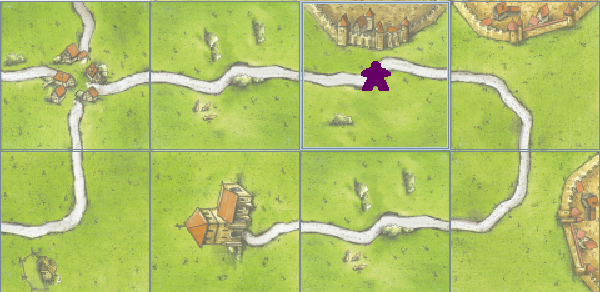
\includegraphics[scale=.4]{images/StradaMeeple.png}}
    \hfill
    \subfigure[Monastero]{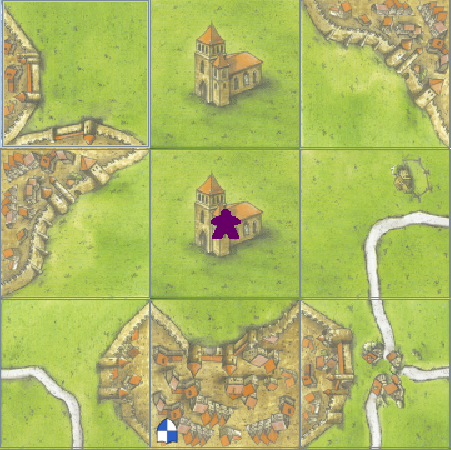
\includegraphics[scale=.4]{images/MonasteroMeeple.png}}
    % \hfill
    % \subfigure[Prateria]{\includegraphics[scale=.07]{images/PrateriaMeeple.png}}
    \caption{Tipi di strutture}
\end{figure}

È possibile che due strutture in cui sono piazzati due o più seguaci (anche dello stesso colore) vengano unite tramite una tessera di congiunzione. In questo caso alla chiusura della struttura il giocatore che avrà la maggioranza di seguaci otterrà i punti vincendo su tutti gli altri. In caso di pareggio ogni giocatore otterrà la totalità dei punti.

Le difficoltà primarie sono:
\begin{itemize}
    \item rappresentare il concetto di tessera coerentemente con la sua rappresentazione grafica
    \item rappresentare il concetto di struttura
    \item unire strutture dello stesso tipo
    \item fare il conteggio dei punti rispettando le regole del gioco
\end{itemize}

